
\documentclass[conference,compsoc]{IEEEtran}
\usepackage[utf8]{inputenc}
\usepackage{natbib}
\usepackage{graphicx}
\usepackage{amsmath}
\usepackage{amssymb}
\usepackage{hyperref}




% *** CITATION PACKAGES ***
%
\ifCLASSOPTIONcompsoc
  % IEEE Computer Society needs nocompress option
  % requires cite.sty v4.0 or later (November 2003)
  \usepackage[nocompress]{cite}
\else
  % normal IEEE
  \usepackage{cite}
\fi



% correct bad hyphenation here
\hyphenation{op-tical net-works semi-conduc-tor}


\begin{document}
%
% paper title
% Titles are generally capitalized except for words such as a, an, and, as,
% at, but, by, for, in, nor, of, on, or, the, to and up, which are usually
% not capitalized unless they are the first or last word of the title.
% Linebreaks \\ can be used within to get better formatting as desired.
% Do not put math or special symbols in the title.
\title{Proyecto Análisis de Algoritmos}


% author names and affiliations
% use a multiple column layout for up to three different
% affiliations
\author{\IEEEauthorblockN{María José Mendoza Rincón}
\IEEEauthorblockA{Pontificia Universidad Javeriana\\
Bogotá, Colombia\\
Email: m.mendozar@javeriana.edu.co}
\and
\IEEEauthorblockN{David Leonardo Velasco Zambrano}
\IEEEauthorblockA{Pontificia Universidad Javeriana\\
Bogotá, Colombia\\
Email: velasco-d@javeriana.edu.co}
}
% make the title area
\maketitle

% As a general rule, do not put math, special symbols or citations
% in the abstract
\begin{abstract}
En el siguiente artículo se presentan tres problemas. El primero relacionado con programación lineal donde se determina dónde ubicar un conjunto de tiendas con el fin de minimizar la distancia de los clientes a las mismas. El siguiente problema se trata de encontrar el árbol de expansión mínimo dadas unas restricciones en la cantidad de aristas de cierto tipo. Finalmente, en el tercer problema se busca el clique máximo en un grafo de Hamming. Para cada problema se presenta la descripción detallada, la fundamentación teórica, las soluciones propuestas y la solución implementada.
\end{abstract}

\IEEEpeerreviewmaketitle

\section{Introducción}
% no \IEEEPARstart
Un algoritmo es cualquier procedimiento computacional bien definido que toma algún valor o conjunto de valores como entrada y produce algún valor o conjunto de valores como salida. Por lo tanto, un algoritmo es una secuencia de pasos computacionales que transforman la entrada en la salida. Se pueden resolver muchísimos tipos de problemas usando algoritmos, como el manejo de grandes volúmenes de datos en internet, así como el análisis de estos, comercio electrónico, etc. Lo que hace interesante a los algoritmos es que puede haber muchas soluciones para un mismo problema y que tiene aplicaciones prácticas. Por ejemplo, una empresa de transporte que desee encontrar la ruta más corta de un punto a otro para así ahorrar gasolina y tener menor trabajo.[1]


%-----------------------------------------------------------------------------------------------------------------------------------------------------
%PROBLEMA 1
\section{Problema 1}
(LP) Suponga que se planea construir una nueva cadena de tiendas en una ciudad dada, usted tiene identificado una serie de ubicaciones potenciales en diferentes barrios. Además, asuma que la demanda de productos en cada barrio de la ciudad es conocida. Si usted quiere construir exactamente k tiendas, ¿dónde debería localizarlas de forma que minimice la distancia promedio de los clientes? ¿Si en lugar usted dese construir una cantidad variable de tiendas, y el costo de construir una tienda en cada sitio es conocido, ¿dónde debería construir las tiendas de forma que minimice el costo total de la construcción y la distancia promedio de los clientes?


\subsection{Fundamentación Teórica}
\subsubsection{Programación Lineal}

La programación lineal (PL) es una herramienta que ha ahorrado mucho dinero a las compañías, Una aplicación común es el problema general de asignar de la mejor manera, es decir, de forma óptima, recursos limitados a actividades que compiten entre sí por ellos. Explicándolo de otra manera, el problema consiste en elegir el nivel de ciertas actividades que compiten por recursos escasos necesarios para realizarlas. La PL utiliza un modelo matemático para describir el problema. “Lineal” significa que todas las funciones matemáticas del modelo deben ser funciones lineales y “programación” es sinónimo de planeación. En conclusión, la PL involucra la planeación de actividades para obtener un resultado que mejor alcance la meta especificada entre todas las alternativas posibles[2]. Existen muchas áreas en donde se aplica la programación lineal, por ejemplo: inversión, planificación de la producción y control de inventarios, planificación de la mano de obra, planificación de desarrollo urbano y refinación y mezcla de petróleo.[3]


\subsubsection{Problema de la ruta más corta}
Consideremos un $G=(V,E)$, donde cada arista $E=(v_{i}, v_{j})$ tiene un peso asociado $c_{i,j}$. El costo del camino $v_{1} v_{2} ... v_{N}$ es $\sum_{i=1}^{N-1} c_{i,j+1}$. Si el grafo no tuviera pesos en las aristas sería el número de aristas en el camino, es decir, N-1.[4]
Dos de los algoritmos para encontrar la ruta más corta son el algoritmo de Dijkstra, que determina las rutas más cortas ente el nodo origen y los demás nodos del grafo, y el algoritmo de Floyd, que determina la ruta más corta entre dos nodos cualesquiera del grafo.[5]

\subsubsection{Algoritmo de Dijkstra}
Se empieza en un nodo origen y a partir de este se miran todos los nodos adyacentes a él, se escogerá el nodo cuya arista entre el nodo origen y este sea de menor peso. Se realizará el mismo procedimiento, reemplazando el nodo origen por el que se va escogiendo, teniendo en cuenta que se va sumando todo el camino recorrido. Por ejemplo, consideremos un nodo origen A y encontramos que el nodo adyacente con menor peso en la arista que los conecta es el nodo B, ahora miramos los nodos adyacentes a B, entonces comparamos el camino recorrido hacia cada uno de los nodos adyacentes a B, el camino recorrido en este caso será el peso de la arista entre A y B más el peso de la arista entre B y el nodo adyacente. 

Por ejemplo, en el siguiente grafo dirigido escogeremos el V1 como el vértice origen. Comparamos con todos los vértices adyacentes V2 y V4, el de menor peso es v4. Tenemos que el camino más corto es igual a 1, el peso de la arista entre v1 y v4. Miramos los nodos adyacentes a v4: v5, v6 y v7. Se escoge v5 ya que la suma entre v1, v4 y v5 es menor que la suma entre v1, v4 y v6 y que v1 v4 y v7. Continuamos iterando y el resultado se puede ver en la figura 1. [4]

\begin{figure}[h]
    \centering
    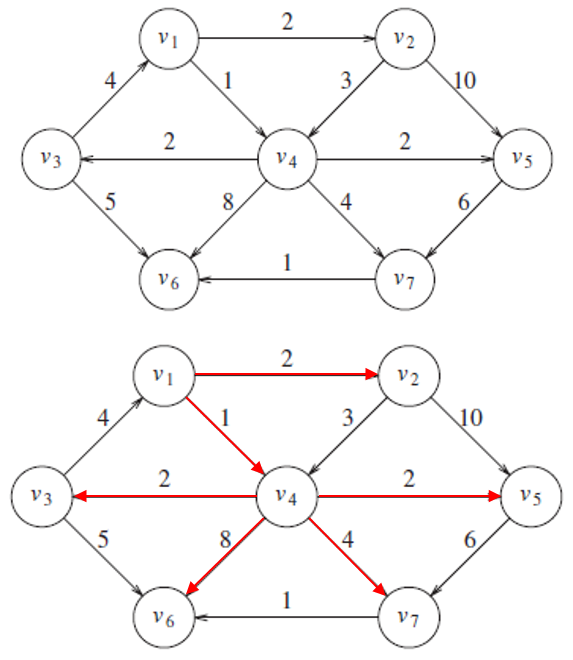
\includegraphics[width=0.25\textwidth]{Problema1/PL1.png}
    \caption{Algoritmo de Dijkstra [4]}
    \label{fig:mesh1}
\end{figure}

\subsubsection{Algoritmo de Floyd}
A diferencia del algoritmo de Dijkstra, el algoritmo de Floyd calcula la distancia entre dos nodos cualesquiera del grafo. El algoritmo representa el grafo de n nodos como una matriz cuadrada  con n filas y n columnas. La entrada (i,j) de la matriz da la distancia $d_{ij}$ del nodo i al nodo j. La idea del algoritmo de Floyd es que dados tres nodos i,j y k con los respectivos pesos entre las tres aristas como muestra la imagen, es más corto llegar de j a i pasando por k si:
$$d_{ik} + d_{kj} <d_{ij}$$
Entonces se reemplaza la ruta directa i->j con la ruta indirecta i->k->j. [3]

\begin{figure}[h]
    \centering
    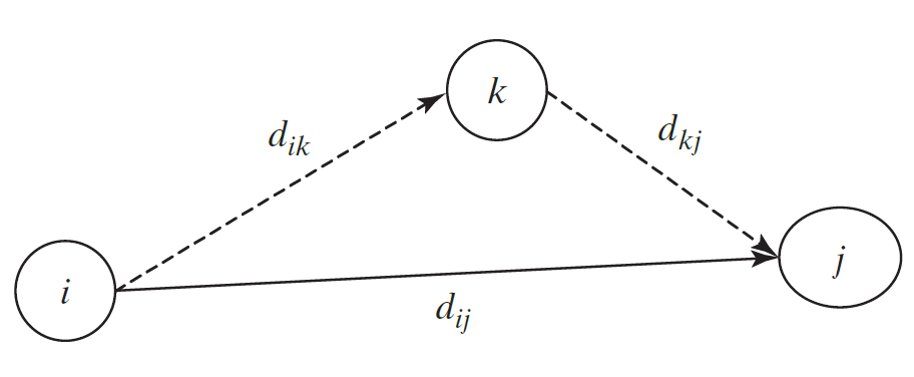
\includegraphics[width=0.25\textwidth]{Problema1/PL2.png}
    \caption{Algoritmo de Floyd[3]}
    \label{fig:mesh1}
\end{figure}


\subsubsection{Facility Location Problem}
Los Facility Location Problem  se ocupan de seleccionar la ubicación de una instalación para satisfacer mejor las restricciones exigidas. El problema consiste normalmente en seleccionar una ubicación para una fábrica que minimice las distancias totales ponderadas de proveedores y clientes, donde las ponderaciones son representativas de la dificultad de transportar materiales. La solución a este problema da la opción de mayor beneficio que satisface más eficientemente las necesidades de todos los consumidores [6].

\subsubsection{Fermat-Weber Problem}
El Fermat-Weber Problem fue uno de los primeros Facility Location Problem que se propusieron, fue realizado a principios del siglo XII. Se considera como “mediana geométrica de tres puntos” es una versión del Facility Location Problem donde se asume que los costos de transporte por distancia son los mismos para todos los destinos. 
El matemático francés Pierre de Fermat lo presento de la siguiente manera:
“Dados tres puntos en un plano, se debe encontrar un cuarto punto tal que la suma de sus distancias a los tres puntos es la mas pequeña como sea posible” [6]


\subsection{Descripción detallada}
El problema consiste en un grupo de barrios que se modelan mediante un grafo, y tienen conexiones entre sí, con una distancia en las aristas entre vértices, se desea poner un número K de tiendas de manera que se minimice la distancia promedio entre clientes, además en otro caso, construir una tienda en un barrio tiene un costo diferente, de manera que se tiene que minimizar la distancia de los clientes a las tiendas y el costo de construcción.
Este es un problema que puede llegar a ser NP-Hard para resolver de manera óptima, y se asimila al “Weber Problem” pero en ese caso solo se tiene que ubicar una tienda, no K tiendas.

\subsection{Solución Propuesta}
La solución que se propone consiste en una adaptación del algoritmo de Warshall, consiste en un principio en crear la matriz de Warshall para saber cuál es el mejor primer nodo para poner la primera tienda, sumando las distancias que necesitan todos los barrios en llegar a uno y hallando el mínimo.
Con esto se crea una matriz que va a tener cada nodo, la distancia a la tienda más cercana y cuál es la tienda más cercana. A partir de aquí se va a iterar con todos los nodos, simulando que la siguiente tienda se pone ahí, y se actualiza la matriz de la distancia mínima a una tienda, y el nodo que reduzca en mayor medida la distancia total es donde se va a poner la siguiente tienda.
Este procedimiento se repite hasta que se llegue a las K tiendas deseadas, en el caso en que las tiendas son variables y se tiene un costo de construcción, se debe realizar una ponderación de factores entre la distancia y el costo de construcción y así decidir cuál barrio es el que trae mejor beneficio para construir una tienda.

\subsection{Instancia del Problema y Solución}

Para el ejemplo se tiene una ciudad con 6 barrios y se desea poner 2 tiendas, el grafo inicial es 

\begin{figure}[h] 
    \centering
    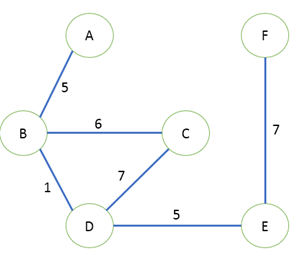
\includegraphics[width=0.25\textwidth]{Problema1/p1.png}
    \caption{Grafo inicial}
    \label{fig:mesh1}
\end{figure}

$$$$$$$$

Se realiza el algoritmo de Warshall para hallar la distancia mínima entre cada para de vértices
\begin{figure}[h] 
    \centering
    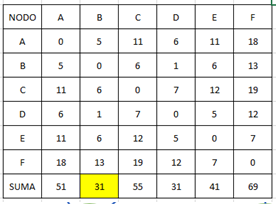
\includegraphics[width=0.25\textwidth]{Problema1/p2.png}
    \caption{Matriz de Warshall}
    \label{fig:mesh1}
\end{figure}

En la suma, el mejor nodo para poner la tienda es el B, debido a que es el central.
Con esto se construye la matriz de distancia a la tienda más cercana

\begin{figure}[h] 
    \centering
    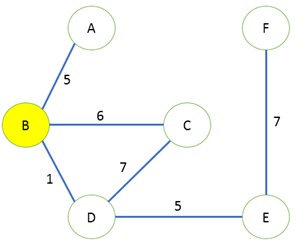
\includegraphics[width=0.20\textwidth]{Problema1/p3.png}
    \caption{Primera tienda seleccionada}
    \label{fig:mesh1}
\end{figure}

\begin{figure}[h] 
    \centering
    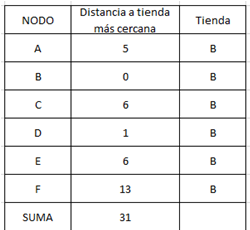
\includegraphics[width=0.20\textwidth]{Problema1/p4.png}
    \caption{Tabla de distancias a la tienda más cercana}
    \label{fig:mesh1}
\end{figure}
Y ahora se realiza la simulación de cada nodo para saber en dónde es mejor poner la siguiente tienda.

\begin{figure}[h]
    \centering
    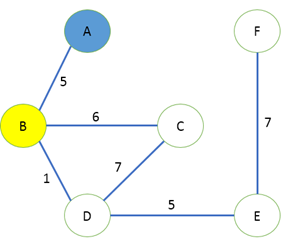
\includegraphics[width=0.20\textwidth]{Problema1/p5.png}
    \caption{Simulación de tienda A }
    \label{fig:mesh1}
\end{figure}

\begin{figure}[h]
    \centering
    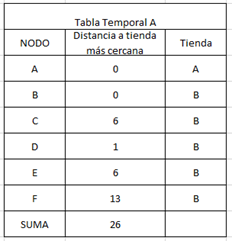
\includegraphics[width=0.20\textwidth]{Problema1/p6.png}
    \caption{Tabla temporal A}
    \label{fig:mesh1}
\end{figure}
$$$$$$$$
Poniendo una tienda en el nodo A, se mejora la distancia en 5

\begin{figure}[h]
    \centering
    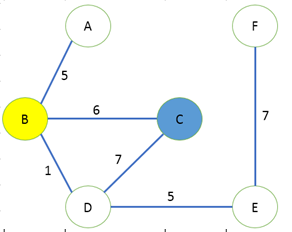
\includegraphics[width=0.20\textwidth]{Problema1/p7.png}
    \caption{ Simulación de tienda C }
    \label{fig:mesh1}
\end{figure}
\begin{figure}[h]
    \centering
    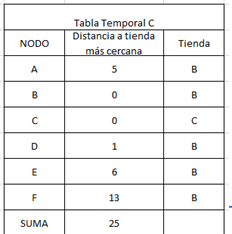
\includegraphics[width=0.20\textwidth]{Problema1/p8.png}
    \caption{Tabla temporal C}
    \label{fig:mesh1}
\end{figure}
$$$$$$$$$$$$$$$$
Poniendo una tienda en el nodo C, la distancia mejora en 6

\begin{figure}[h]
    \centering
    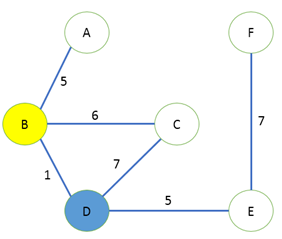
\includegraphics[width=0.20\textwidth]{Problema1/p9.png}
    \caption{ Simulación de tienda D }
    \label{fig:mesh1}
\end{figure}
\begin{figure}[h]
    \centering
    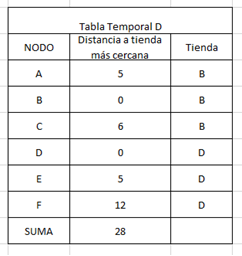
\includegraphics[width=0.20\textwidth]{Problema1/p10.png}
    \caption{Tabla temporal D}
    \label{fig:mesh1}
\end{figure}
$$$$
Poniendo una tienda en el nodo D, la distancia mejora en 3
\begin{figure}[h]
    \centering
    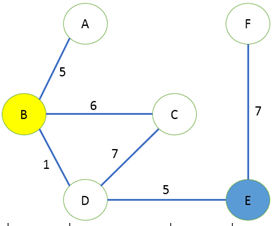
\includegraphics[width=0.20\textwidth]{Problema1/p11.png}
    \caption{ Simulación de tienda E }
    \label{fig:mesh1}
\end{figure}
\begin{figure}[h]
    \centering
    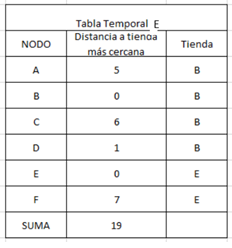
\includegraphics[width=0.20\textwidth]{Problema1/p12.png}
    \caption{Tabla temporal E}
    \label{fig:mesh1}
\end{figure}
$$$$
Poniendo una tienda en el nodo E, se mejora la distancia en 12.
\begin{figure}[h]
    \centering
    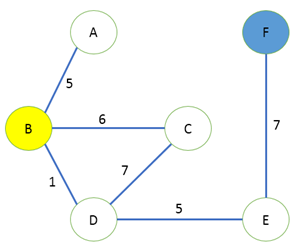
\includegraphics[width=0.20\textwidth]{Problema1/p13.png}
    \caption{ Simulación de tienda F }
    \label{fig:mesh1}
\end{figure}
\begin{figure}[h]
    \centering
    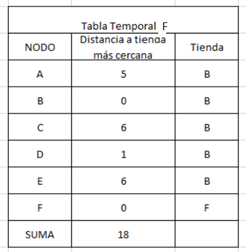
\includegraphics[width=0.20\textwidth]{Problema1/p14.png}
    \caption{Tabla temporal F}
    \label{fig:mesh1}
\end{figure}
$$$$
Poniendo una tienda en el nodo F, la distancia se mejora en 13.
Cuando se termina de recorrer los nodos, se elige el que mejoró en mayor medida la distancia, en este caso fue F.
Se escoge F como la siguiente tienda, y acaba el algoritmo.

\begin{figure}[h]
    \centering
    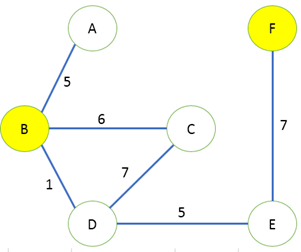
\includegraphics[width=0.25\textwidth]{Problema1/p15.png}
    \caption{Grafo con tiendas seleccionadas}
    \label{fig:mesh1}
\end{figure}
\begin{figure}[h]
    \centering
    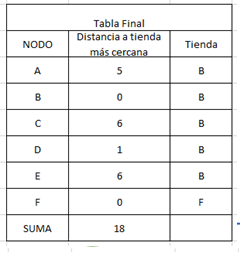
\includegraphics[width=0.25\textwidth]{Problema1/p16.png}
    \caption{Tabla Final}
    \label{fig:mesh1}
\end{figure}

\subsection{Solución implementada}
En primera instancia, en la solución implementada se utilizó Floyd Warshall para calcular la distancia entre todos los nodos. Luego se hacen todas las posibles combinaciones de tiendas, es decir, si se quieren poner 2 tiendas se miran todas las combinaciones de 2 tiendas posibles, y la menor es la mejor opción. 
Ejemplo:
La siguiente es la matriz de adyacencia inicial y se quiere encontrar dos tiendas que minimicen la distancia a los clientes.
\begin{figure}[h]
    \centering
    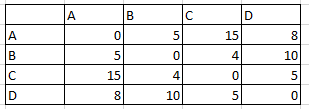
\includegraphics[width=0.25\textwidth]{Problema1/p17.png}
    \caption{Matriz de adyacencia inicial}
    \label{fig:mesh1}
\end{figure}

Se ejecuta el algoritmo de Floyd Wharshall. 
\begin{figure}[h]
    \centering
    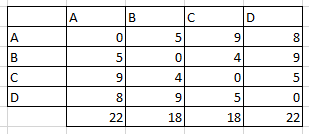
\includegraphics[width=0.25\textwidth]{Problema1/p18.png}
    \caption{Matriz de adyacencia - FLoyd Wharshall}
    \label{fig:mesh1}
\end{figure}

Se realiza una simulación si se colocara una tienda en A y la otra en cada uno de los nodos
\begin{figure}[h]
    \centering
    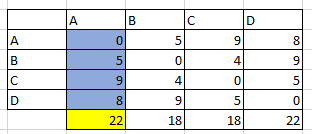
\includegraphics[width=0.25\textwidth]{Problema1/p19.png}
    \caption{Matriz de adyacencia - A}
    \label{fig:mesh1}
\end{figure}
\begin{figure}[h]
    \centering
    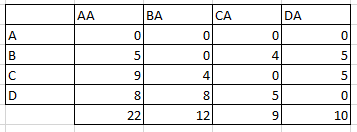
\includegraphics[width=0.25\textwidth]{Problema1/p110.png}
    \caption{Matriz de adyacencia - A}
    \label{fig:mesh1}
\end{figure}
$$$$
Se realiza una simulación si se colocara una tienda en B y la otra en cada uno de los nodos.
$$$$$$$$

\begin{figure}[h]
    \centering
    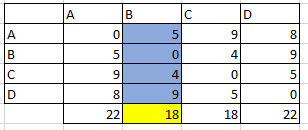
\includegraphics[width=0.25\textwidth]{Problema1/p111.png}
    \caption{Matriz de adyacencia - B}
    \label{fig:mesh1}
\end{figure}
\begin{figure}[h]
    \centering
    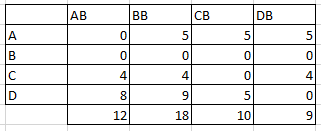
\includegraphics[width=0.25\textwidth]{Problema1/p112.png}
    \caption{Matriz de adyacencia - B}
    \label{fig:mesh1}
\end{figure}
$$$$$$$$
Se realiza una simulación si se colocara una tienda en C y la otra en cada uno de los nodos.
$$$$
\begin{figure}[h]
    \centering
    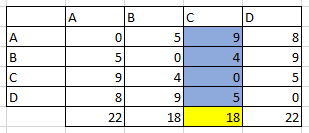
\includegraphics[width=0.25\textwidth]{Problema1/p113.png}
    \caption{Matriz de adyacencia - C}
    \label{fig:mesh1}
\end{figure}
\begin{figure}[h]
    \centering
    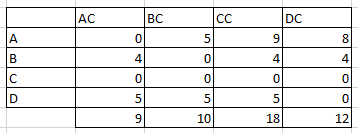
\includegraphics[width=0.25\textwidth]{Problema1/p114.png}
    \caption{Matriz de adyacencia inicial - C}
    \label{fig:mesh1}
\end{figure}
$$$$$$$$$$$$$$$$
Se realiza una simulación si se colocara una tienda en D y la otra en cada uno de los nodos.
$$$$$$$$$$$$
\begin{figure}[h]
    \centering
    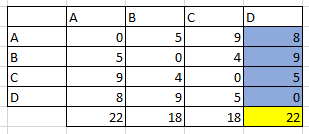
\includegraphics[width=0.25\textwidth]{Problema1/p115.png}
    \caption{Matriz de adyacencia - D}
    \label{fig:mesh1}
\end{figure}
\begin{figure}[h]
    \centering
    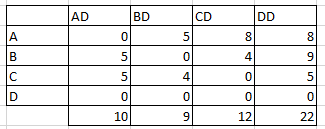
\includegraphics[width=0.25\textwidth]{Problema1/p116.png}
    \caption{Matriz de adyacencia - D}
    \label{fig:mesh1}
\end{figure}
$$$$$$$$$$$$
El mejor caso es poner una tienda en D y otra en B, minimiza la distancia a 9 al igual que poner una tienda en A y otra en C.
$$$$
\begin{figure}[h]
    \centering
    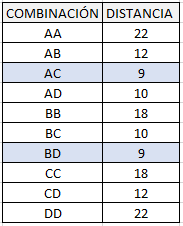
\includegraphics[width=0.25\textwidth]{Problema1/p117.png}
    \caption{Resultados}
    \label{fig:mesh1}
\end{figure}

En caso de necesitarse otra tienda se realizan más simulaciones con todas las combinaciones ABC, ABD, BCD, etc. 
ANÁLISIS:
Se generaron matrices aleatorias cambiando el tamaño hasta un número n dado. Por cada matriz se ejecutó el algoritmo con distinta cantidad de tiendas y se calculó el tiempo. Para un n=8 la gráfica de tiempo dio así:

\begin{figure}[h]
    \centering
    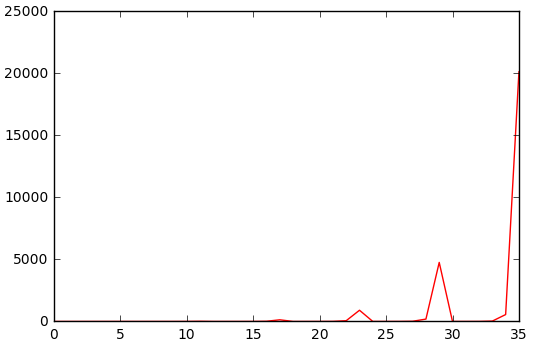
\includegraphics[width=0.25\textwidth]{Problema1/p118.png}
    \caption{Gráfica de tiempos}
    \label{fig:mesh1}
\end{figure}

Cada uno de los picos representa el máximo tiempo de ejecución de grafos, variando su tamaño y el número de tiendas.
Se observan 4 picos, para grafos de tamaño 5, 6, 7 y 8


%-----------------------------------------------------------------------------------------------------------------------------------------------------
%PROBLEMA 2
\section{Problema 2}
(MST). Dado un grafo G = (V, E) con n vértices y m aristas. (El grafo podría representar una red telefónica). Cada arista es coloreada azul o roja. También está dado un parámetro k como parte de la entrada. Proponga un algoritmo que encuentre un árbol de expansión sobre G con exactamente k aristas azules, y exactamente n-k-1 aristas rojas. Determine el tiempo de ejecución del algoritmo y muestre que es correcto.

\subsection{Fundamentación Teórica}
\subsubsection{Árboles}
Un árbol es una colección de nodos. La colección puede estar vacía; De lo contrario, un árbol consta de un nodo distinguido, r, llamado la raíz, y cero o más árboles (sub) no vacíos T1, T2,. . . , Tk, cada una de cuyas raíces están conectadas por una arista dirigida desde r. Se dice que la raíz de cada subárbol es un hijo de r, y r es el padre de cada raíz de subárbol.[4]
\begin{figure}[h]
    \centering
    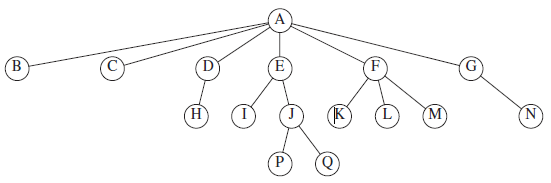
\includegraphics[width=0.25\textwidth]{Problema2/M1.png}
    \caption{Árbol [4]}
    \label{fig:mesh1}
\end{figure}
\subsubsection{Grafos}
Un gráfico G = (V, E) consiste en un conjunto de vértices, V, y un conjunto de aristas, E. Cada arista es un par (v, w), donde v, w ∈ V. Si el par está ordenado, entonces el gráfico está dirigido. El vértice w es adyacente a v si y sólo si (v, w) ∈ E. En un gráfico no dirigido con arista (v, w), y por lo tanto (w, v), w es adyacente a v y v es adyacente a w. A veces una arista tiene un tercer componente, conocido como un peso o un costo.[4]

Un camino en un grafo es una secuencia de vértices w1, w2, w3,. . . , WN tal que (wi, wi + 1) ∈ E para 1 ≤ i <N. La longitud del camino es el número de aristas en la trayectoria, que es igual a N - 1. Permitimos una trayectoria desde un vértice a sí mismo; Si este camino no contiene aristas, entonces la longitud de la trayectoria es 0. Un grafo no dirigido se conecta si hay una trayectoria de cada vértice a cada otro vértice.[4]

\begin{figure}[h]
    \centering
    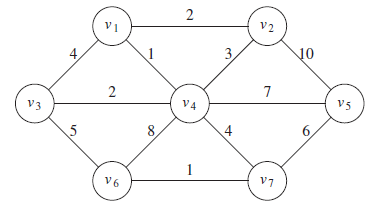
\includegraphics[width=0.25\textwidth]{Problema2/M2.png}
    \caption{Grafo [4]}
    \label{fig:mesh1}
\end{figure}
\subsubsection{Árbol de expansión mínimo}
Un árbol de expansión mínimo de un grafo no dirigido G es un árbol formado a partir de las aristas del grafo que conecta todos los vértices de G con el costo total más bajo. Existe un árbol de expansión mínimo si y sólo si G está conectado. 
El árbol expansión mínimo es un árbol porque es acíclico, es de expansión porque cubre cada vértice, y es mínimo por la razón obvia.

\begin{figure}[h]
    \centering
    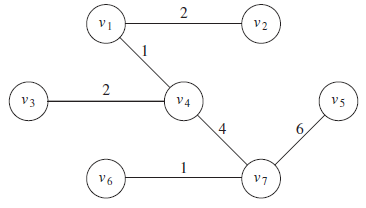
\includegraphics[width=0.25\textwidth]{Problema2/M3.png}
    \caption{Árbol de expansión mínimo[4]}
    \label{fig:mesh1}
\end{figure}


\subsubsection{Algoritmo de Kruskal}
Una forma de calcular el árbol de expansión mínimo es seleccionar continuamente las aristas en orden de menor peso y aceptar una arista si no genera un ciclo.
El algoritmo de Kruskal mantiene un bosque: una colección de árboles. Inicialmente, hay |V| árboles de un solo nodo. La adición de una arista combina dos árboles en uno. Cuando el algoritmo termina, sólo hay un árbol, y éste es el árbol de expansión mínimo.[4]


\subsection{Descripción detallada}
El problema parte de un grafo que tiene X aristas azules y Y aristas rojas, para que el problema sea realizable se debe tener en cuenta que el parámetro K de entrada debe ser menor o igual X. Para poder hallar el árbol de expansión mínimo actualmente existen varios algoritmos, los más reconocidos son el algoritmo de Kruskal y Prim, pero ninguno de estos contempla el hecho de diferentes tipos de aristas, pero se podrían llegar a adaptar para este problema específico.
El principal problema que se tiene es que no se puede determinar una fórmula para determinar si el grafo tiene un árbol de expansión con un K determinado. En todos los casos el número total de aristas que va a tener el árbol es de N – 1, esto corresponde a la suma entre las aristas azules K y las rojas N – K – 1.


\subsection{Solución Propuesta}
Se va a adaptar el algoritmo de Kruskal, para esto, al principio del algoritmo se le va a asignar peso 1 a todas las aristas del grafo y se va a escoger una combinación aleatoria. Se deben llevar 2 contadores, el número de aristas rojas y el número de aristas rojas que se han escogido. Se mira la primera arista en la lista y se verifica si al unir sus vértices se forma un ciclo, si no se forma se unen los dos árboles y en caso contrario se pasa a la siguiente arista, y se actualizan los contadores según corresponde. Si un contador llega al número de aristas que se necesita de ese color, el peso de las aristas de ese mismo color se pone en 1000 (un número muy grande), y se vuelve a ordenar la lista de las aristas, dejando al final las del color que ya no se necesitan. Se repite el proceso hasta acabar el árbol de expansión y al final se suma el peso de las aristas, si la suma es N – 1, el árbol es correcto y en caso contrario se debe repetir todo el algoritmo con una combinación diferente en la lista inicial de aristas.

\subsection{Instancia del Problema y Solución}


El grafo inicial es el siguiente:

\begin{figure}[h] 
    \centering
    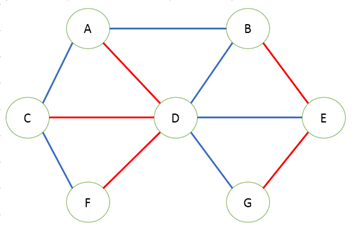
\includegraphics[width=0.25\textwidth]{Problema2/s1.png}
    \caption{Grafo Inicial}
    \label{fig:mesh1}
\end{figure}

Se va a realizar para K = 2
Es decir, se va a tener 2 aristas azules y 4 rojas al final
Al principio del algoritmo se ve así

\begin{figure}[h] 
    \centering
    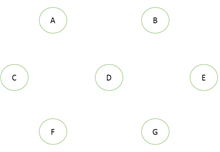
\includegraphics[width=0.25\textwidth]{Problema2/s2.png}
    \caption{Grafo sin aristas}
    \label{fig:mesh1}
\end{figure}
\begin{figure}[h] 
    \centering
    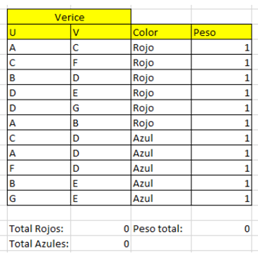
\includegraphics[width=0.25\textwidth]{Problema2/s3.png}
    \caption{Tabla de aristas inicial}
    \label{fig:mesh1}
\end{figure}

$$$$$$$$$$$$
Se elige la primera arista de la lista
\begin{figure}[h] 
    \centering
    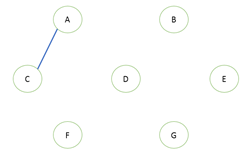
\includegraphics[width=0.25\textwidth]{Problema2/s4.png}
    \caption{Grafo con arista A-C}
    \label{fig:mesh1}
\end{figure}

$$$$
La siguiente arista tampoco tiene problema

\begin{figure}[h] 
    \centering
    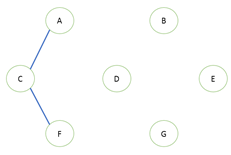
\includegraphics[width=0.25\textwidth]{Problema2/s5.png}
    \caption{Grafo con arista C-F}
    \label{fig:mesh1}
\end{figure}

Como ya se tienen las dos aristas azules necesarias entonces se actualiza la lista de aristas

\begin{figure}[h] 
    \centering
    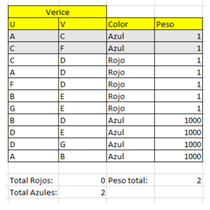
\includegraphics[width=0.25\textwidth]{Problema2/s6.png}
    \caption{Tabla de aristas reorganizado}
    \label{fig:mesh1}
\end{figure}

Se escoge la tercera arista

\begin{figure}[h] 
    \centering
    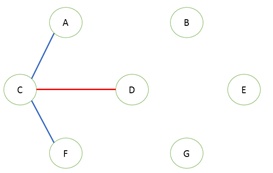
\includegraphics[width=0.25\textwidth]{Problema2/s7.png}
    \caption{Grafo con arista C-D Roja}
    \label{fig:mesh1}
\end{figure}

La cuarta arista y la quinta no se pueden poner porque generaría un ciclo, entonces se escoge la sexta

\begin{figure}[h]
    \centering
    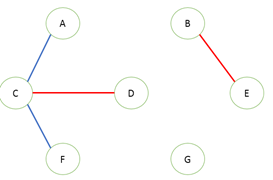
\includegraphics[width=0.25\textwidth]{Problema2/s8.png}
    \caption{Grafo con arista B-E Roja}
    \label{fig:mesh1}
\end{figure}
$$$$$$$$
Se escoge la séptima arista

\begin{figure}[h] 
    \centering
    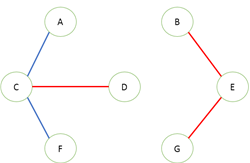
\includegraphics[width=0.25\textwidth]{Problema2/s9.png}
    \caption{Grafo con arista G-E Roja}
    \label{fig:mesh1}
\end{figure}

Y por obligación se escoge la octava arista, que es incorrecta

\begin{figure}[h] 
    \centering
    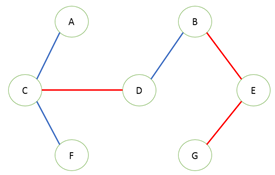
\includegraphics[width=0.25\textwidth]{Problema2/s10.png}
    \caption{Grafo con arista B-D Azul incorrecta}
    \label{fig:mesh1}
\end{figure}

\begin{figure}[h] 
    \centering
    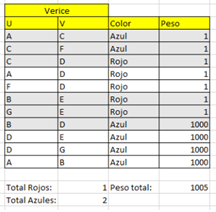
\includegraphics[width=0.25\textwidth]{Problema2/s11.png}
    \caption{Tabla de aristas total incorrecta}
    \label{fig:mesh1}
\end{figure}

El peso correcto debería ser 6, pero el peso total fue 1005, por lo que se escogió una arista azul de más.
Entonces se debe volver a empezar el algoritmo con una combinación de aristas diferente, la lista a seguir es:

\begin{figure}[h] 
    \centering
    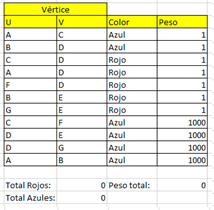
\includegraphics[width=0.25\textwidth]{Problema2/s12.png}
    \caption{Tabla de aristas inicial}
    \label{fig:mesh1}
\end{figure}
$$$$
Se escoge la primera y segunda arista
\begin{figure}[h] 
    \centering
    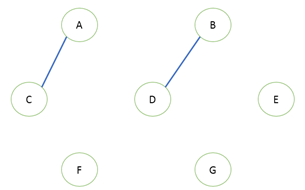
\includegraphics[width=0.25\textwidth]{Problema2/s13.png}
    \caption{Grafo con aristas A-C y B-D}
    \label{fig:mesh1}
\end{figure}

Se actualiza la tabla y se reordena
\begin{figure}[h] 
    \centering
    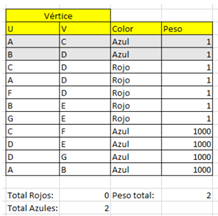
\includegraphics[width=0.25\textwidth]{Problema2/s14.png}
    \caption{Tabla de aristas reordenada}
    \label{fig:mesh1}
\end{figure}

Se escoge la tercera arista
\begin{figure}[h] 
    \centering
    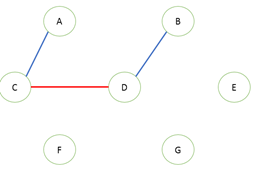
\includegraphics[width=0.25\textwidth]{Problema2/s15.png}
    \caption{Grafo con arista C-D Roja}
    \label{fig:mesh1}
\end{figure}

La cuarta arista forma un ciclo entonces se salta y se toma la quinta

\begin{figure}[h] 
    \centering
    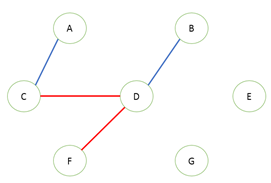
\includegraphics[width=0.25\textwidth]{Problema2/s16.png}
    \caption{Grafo con arista D-F Roja}
    \label{fig:mesh1}
\end{figure}
$$$$
Se toma la quinta y sexta arista
\begin{figure}[h] 
    \centering
    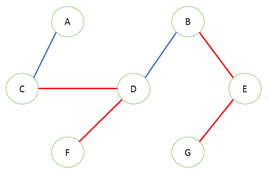
\includegraphics[width=0.25\textwidth]{Problema2/s17.png}
    \caption{Grafo con aristas B-E y E-G Rojas}
    \label{fig:mesh1}
\end{figure}
\begin{figure}[h] 
    \centering
    \includegraphics[width=0.25\textwidth]{Problema2/s18.png}
    \caption{Tabla de aristas final correcta}
    \label{fig:mesh1}
\end{figure}

El peso total es 6 correspondiente a N-1, se concluye que el árbol de expansión es correcto y el algoritmo finaliza.

\subsection{Solución implementada}
El algoritmo implementado para encontrar el árbol de expansión mínima de un grafo con k aristas azules y n-k-1 aristas rojas recibe el número total de nodos, la matriz de adyacencia en cuanto a pesos y colores, las cuales son simétricas y el número k. El procedimiento que realiza es el siguiente:
Se elige el primer nodo, es decir, el de la primera fila de la matriz, y se buscan los nodos adyacentes que tengan menor peso en la arista. Esto se hace tanto para aristas rojas como aristas azules, por lo tanto, tendremos dos nodos, el de menor peso con arista azul y el de menor peso con arista roja. Luego se buscan dos nodos adyacentes con menores pesos, y así sucesivamente. Es importante aclarar que, solamente se miran los nodos adyacentes que ya fueron visitados. Se hace este mismo proceso para otro nodo que no se haya visitado.
El algoritmo va llevando la cuenta de aristas azules y rojas va acumulando. Cuando llega a k aristas azules y n-k-1 aristas rojas revisa el peso total, si este es el primero en encontrarse se guarda en una variable global, así como el árbol de expansión mínima, si no lo es y es menor que el que se encuentra en la variable global, actualiza el valor y guarda el nuevo árbol de expansión mínima que encontró.
Vamos a verlo con un ejemplo:
Tenemos el siguiente grafo de 6 nodos y k=2 (2 aristas azules y 6-2-1=3 aristas rojas):
\begin{figure}[h] 
    \centering
    \includegraphics[width=0.25\textwidth]{Problema2/p21.png}
    \caption{Tabla de aristas final correcta}
    \label{fig:mesh1}
\end{figure}

El primer nodo sería el número 1, se miran los nodos adyacentes de menor valor que tengan arista azul y roja. Y se marca como visitado el nodo 1.
\begin{figure}[h] 
    \centering
    \includegraphics[width=0.25\textwidth]{Problema2/p22.png}
    \caption{Tabla de aristas final correcta}
    \label{fig:mesh1}
\end{figure}

Si continuamos con el nodo 2, como solo se ha visitado el nodo 1, es el único nodo adyacente que hay. Se marca como visitado el nodo 2 y se continua con otro nodo que no se haya visitado, por ejemplo, el nodo 3. Se miran los nodos adyacentes al nodo 3 que ya hayan sido visitados. Como ambas aristas son azules, se escoge el de menor peso en la arista que sería el nodo 2. 
El primer nodo sería el número 1, se miran los nodos adyacentes de menor valor que tengan arista azul y roja. Y se marca como visitado el nodo 1.
\begin{figure}[h] 
    \centering
    \includegraphics[width=0.25\textwidth]{Problema2/p23.png}
    \caption{Tabla de aristas final correcta}
    \label{fig:mesh1}
\end{figure}
$$$$$$$$$$$$$$$$$$$$$$$$$$$$
Luego con cada uno de los dos nodos encontrados se realiza lo mismo hasta encontrar el árbol de expansión mínima con k aristas azules y n-k-1 aristas rojas, que en este ejemplo sería el siguiente:  
\begin{figure}[h] 
    \centering
    \includegraphics[width=0.25\textwidth]{Problema2/p24.png}
    \caption{Tabla de aristas final correcta}
    \label{fig:mesh1}
\end{figure}

Como se dijo anteriormente, puede que el algoritmo encuentre más de un árbol que cumpla las condiciones de la cantidad de aristas azules y rojas, para esto, la solución final es el árbol que la suma de sus aristas sea la menor.
ANÁLISIS:
El análisis se realizó implementando un método que genera matrices aleatoriamente hasta un tamaño n indicado. Para cada matriz se ejecuta el algoritmo con diferentes k. Se toma el tiempo que tarda con cada ejecución y se grafican los tiempos. Con n=30 la gráfica que resultó fue:
\begin{figure}[h] 
    \centering
    \includegraphics[width=0.25\textwidth]{Problema2/p25.png}
    \caption{Tabla de aristas final correcta}
    \label{fig:mesh1}
\end{figure}
%-----------------------------------------------------------------------------------------------------------------------------------------------------
%PROBLEMA 3
\section{Problema 3}

La distancia de Hamming dist(u,v) entre dos vectores binarios $v = (v_{1} , . . . , v_{n} ) $and$ w = (w_{1} , . . . , w_{n} )$ es el número de índices k tal que $v_{k} \neq w_k$. Una pregunta fundamental en la teoría de la codificación es determinar el número 
$$A(n, d) = max |{S ⊂ {0, 1} n | dist(u, v) ≥ d for all distinct u, v ∈ S}|$$, 
el máximo número de vectores binarios de longitud n que uno puede encontrar tal que dos vectores diferentes tienen una distancia de Hamming ≥ d.  Por ejemplo, A(5, 4) = 2. 
El grafo de Hamming H(n, d) = (V, E) es el gráfo con $2^{n}$ vertices V dados por cadenas binarias de longitud n. Nosotros tenemos $(u, v) ∈ E$ si y solo si $dist(u, v) ≥ d$. El número A(n,d) coincide con el tamaño de un clique máximo en H(n,d). Encuentre un algoritmo "eficiente"  para calcular el clique máximo en el grafo de Hamming (calcular el clique máximo es un problema NP-difícil).

\subsection{Fundamentación Teórica}
\subsubsection{Distancia de Hamming}

La distancia de Hamming es un número que representa la diferencia entre dos cadenas. Por ejemplo, la distancia de Hamming entre “casa” y “mapa” es 2 ya que se tuvo que cambiar dos letras para convertir una palabra en la otra. En caso de tener vectores binarios, la distancia de Hamming son los bits que cambian de un grupo de bits a otro grupo de bits. Por ejemplo, si tenemos un bit 0 y se cambia a 1, la distancia sería 1, lo mismo si cambia de 0 a 1.

Podemos representar la distancia de Hamming para vectores binarios en un grafo, en el cual cada nodo será un vector binario y las aristas representarán un paso de distancia. Como podemos ver en la siguiente imagen: el grafo respectivo para vectores binarios de longitud 3. Para hallar la distancia de Hamming con ayuda del grafo basta con encontrar el camino más corto entre los dos nodos, y la cantidad de aristas recorridas será la distancia de Hamming. [7]


\begin{figure}[h]
    \centering
    \includegraphics[width=0.25\textwidth]{Problema3/M4.png}
    \caption{Distancia de Hamming[7]}
    \label{fig:mesh1}
\end{figure}


\subsubsection{NP-completo}
La clase P consiste en aquellos problemas que son solubles en tiempo polinomial. Más específicamente, son problemas que pueden resolverse en el tiempo $O (n^{k})$ para alguna constante k, donde n es el tamaño de la entrada al problema.

La clase NP consiste en aquellos problemas que son "verificables" en tiempo polinomial. Esto significa que, si de alguna manera se nos dio un "certificado" de una solución, entonces podríamos verificar que el certificado es correcto en tiempo polinomial en el tamaño de la entrada a el problema.
Los problemas NP-completos surgen en diversos dominios: lógica booleana, gráfos, aritmética, diseño de red, conjuntos y particiones, almacenamiento y recuperación, secuenciación y programación, programación matemática, álgebra y teoría numérica, juegos y puzzles, autómatas y teoría del lenguaje, optimización de programas , biología, química, física, etc [1]. Uno de los problemas mas conocidos NP-Completo es el problema Clique:

\subsubsection{Clique}
CLIQUE = {(G,K) : G es un grafo que contiene un clique  de tamaño k

Un clique en un grafo no dirigido G= (V,E), en el cual V={1,2,…,n} es el conjunto de los vértices del grafo y E es el conjunto de aristas, es un sub conjunto V ⊆ V de vértices en los cuales cada par de ellos está conectado por una arista en E. Un clique es parcial si este forma parte de otro clique, de otra forma es máximo
\begin{figure}[h]
    \centering
    \includegraphics[width=0.25\textwidth]{Problema3/M5.png}
    \caption{Clique Maximo[8]}
    \label{fig:mesh1}
\end{figure}

\subsubsection{Algoritmo Bron-Kerbosch}
El algoritmo Bron-Kerbosch utiliza el paradigma recursivo backtracking para enumerar todos los cliques máximos en un grafo. En todo momento se mantienes tres listas: P,W y X. Al inicio R y X están vacíos mientras que P contiene todos los vértices del grafo. Luego R contiene los resultados temporales, es decir, el conjunto de vértices que están conectados con todos los vértices en P y se pueden añadir a P para formar un clique mayor, P el conjunto de candidatos posibles y  X contiene los vértices que están conectados con todos los vértices en P pero se excluyen de ser agregados en P porque todos los cliques que contienen vértices en X ya han sido enumerados en un ciclo de recursión diferente.[9][10]
El algoritmo funciona de la siguiente manera:
Se elige un vértice v desde P para expandir. Se añade v a R y se elimina a sus no vecinos de P y X. Luego se elije otro vértice del nuevo conjunto P y se repite el proceso. Se continua hasta que P esté vacío. Una vez que P está vacío, si X está vacío, se reporta que el contenido de R contiene un clique máximo (si no es así, R contiene un subconjunto de un clique que ya se había encontrado). Ahora se retrocede hasta el último vértice escogido, se restaura P, R y X tal como estaban antes de la elección, se quita el vértice de P y se añade a X, luego se expande al siguiente vértice. Si no hay más vértices en P, entonces se retrocede al nivel superior [9][10]. La complejidad de este algoritmo es $O(3^{(n/3)})$ [11]


\subsection{Descripción detallada}
El grafo de Hamming se construye a partir de dos parámetros, N y D. N a la cantidad de bits que tendrán los vértices, y D a la distancia mínima que deben tener dos vértices para que exista una arista entre ellos, el problema consiste en encontrar el clique de máximo tamaño que se encuentre en el grafo, para esto ya existen algoritmos como el de Bron-Kerbosch que consiste en ir uniendo cliques de tamaño mínimo hasta que no quede elementos sin mezclar, pero este al ser un problema específico se puede mirar desde un enfoque diferente, porque al tener todos los nodos algo en común, el ser binarios, se puede encontrar de otra manera el clique máximo, incluso sin recorrer el árbol.

\subsection{Solución Propuesta}

Este problema se va a abordar recorriendo cada uno de los vértices del grafo. Para cada uno de ellos se recorrerá la lista de los vértices unidos por una arista y se hará una comparación entre ellos si también están conectados entre sí, teniendo cada vez una lista más pequeña, y cuando se acabe la lista se debe mirar el siguiente nodo de la penúltima lista y compararlo con todos los demás para saber si existe un clique más grande, este algoritmo se ilustra mejor con un ejemplo.
Se sabe desde un principio para un grafo de Hamming H(n,d) se pasa una distancia 1, el clique máximo va a ser de tamaño n, y consiste de todos los vértices del grafo, debido a que todos los vértices tienen entre si una distancia mayor o igual a 1.

\subsection{Instancia del Problema y Solución}

Grafo de Hamming H(3,1)

\begin{figure}[h] 
    \centering
    \includegraphics[width=0.25\textwidth]{Problema3/t1.png}
    \caption{Grafo de Hamming de 3 bits}
    \label{fig:mesh1}
\end{figure}

Como la distancia es 1, se puede inferir que el tamaño del clique máximo es n, es decir 8, conformado por todos los vértices del grafo.

Ejemplo

Se va a partir con el grafo de Hamming H(2,2)
\begin{figure}[h] 
    \centering
    \includegraphics[width=0.25\textwidth]{Problema3/t2.png}
    \caption{Grafo de Hamming de 2 bits}
    \label{fig:mesh1}
\end{figure}
$$$$$$$$$$$$$$$$$$$$
La matriz que representa la distancia de haming es la siguiente:
$$$$
\begin{figure}[h] 
    \centering
    \includegraphics[width=0.25\textwidth]{Problema3/t3.png}
    \caption{Matriz de distancia de Hamming}
    \label{fig:mesh1}
\end{figure}
$$$$$$$$
Comenzamos por tomar el primer vértice 00
Tomamos la lista de nodos cuya distancia es mayor o igual a 2, es decir 11
Al solo tener un elemento, el clique formado por 00 y 11 es de tamaño 2

Luego se recorre el vértice 01, se toma la lista de vértices cuya distancia es mayor o igual a 2, compuesta por 10. Al solo tener un elemento en la lista, se concluye que es un clique de tamaño 2.
Se repite el algoritmo para los otros dos nodos, al final se tendrán 4 cliques de tamaño 2 y eliminando los repetidos se terminarán con 2.
El clique máximo del grafo es de 2 y está compuesto por {00,11} o {01,10}.

\subsection{Solución implementada}

Primero se arma el grafo de hamming. Para esto se generan todas las posibles combinaciones haciendo uso de la librería Itertools y por cada una se crea un nodo. Según la distancia ingresada, se agregan las aristas entre los nodos.
Luego se encuentran todos los cliques. La librería networkx tiene un método que retorna una lista con todos los cliques. El método es: find\_cliques(G), donde G es el grafo de Hamming, basado en el algoritmo de Bron y Kerbosch [12], explicado en la sección 4.1.4.

Para N=4 (cantidad de bits que tendrán los vértices) y D=2 (distancia mínima que deben tener dos vértices para que exista una arista entre ellos) el grafo de hamming luce así:
\begin{figure}[h] 
    \centering
    \includegraphics[width=0.25\textwidth]{Problema3/p31.png}
    \caption{Matriz de distancia de Hamming}
    \label{fig:mesh1}
\end{figure}

El tamaño del clique máximo es 8.
\begin{thebibliography}{1}

\bibitem{IEEEhowto:kopka}
T. H. Cormen, Introduction to algorithms, Cambridge, Massachusetts : MIT Press, 2009.
\bibitem{IEEEhowto:kopka}
F. S. Hillier, Introducción a la investigación de operaciones, México ; Bogotá: McGraw-Hill/Interamericana Editores, 2006.
\bibitem{IEEEhowto:kopka}
H. A. Taha, Investigación de Operaciones, University of Arkansas, Fayetteville: Pearson, 2012
\bibitem{IEEEhowto:kopka}
M. A. Weiss, Data Structures and Algorithm Analysis in C++, Boston, Massachusetts : Pearson, 2014.
\bibitem{IEEEhowto:kopka}
H. A. Taha, Investigación de Operaciones, University of Arkansas, Fayetteville: Pearson, 2012. 
\bibitem{IEEEhowto:kopka}
A. Litoff, «Facility location problems,» 2015. [En línea]. Available: \url{https://optimization.mccormick.northwestern.edu/index.php/Facility_location_problems.}
\bibitem{IEEEhowto:kopka}
R. Invarato, «Jarroba - Hamming,» 2016. [En línea]. Available: \url{https://jarroba.com/hamming/}.
\bibitem{IEEEhowto:kopka}
E. E. P. d. L. P. O. O. Z. Julio C. Ponce, «Algoritmo de Colonia de Hormigas para el Problema del Clique Máximo con un Optimizador Local K-opt,» Hifen,
Uruguaiana, vol. 30, nº 58, 2006.
\bibitem{IEEEhowto:kopka}
A. Conte, «Review of the Bron-Kerbosch algorithm and variations,» University of Glasgow, Glasgow, 2013.
\bibitem{IEEEhowto:kopka}
«Bron Kerbosch Algorithm (BK),» [En línea]. Available: \url{https://static-content.springer.com/esm/art\%3A10.1186\%2F1471-2105-12-440/MediaObjects/12859_2011_5034_MOESM22_ESM.PDF.}
\bibitem{IEEEhowto:kopka}
A. T. H. T. Etsuji Tomitaa, «The worst-case time complexity for generating all maximal cliques and computational experiments,» Science Direct, 2006. 
\bibitem{IEEEhowto:kopka}
NetworkX Developers, «Networkx,» 20 Septiembre 2014. [En línea]. Available:
«Bron Kerbosch Algorithm (BK),» [En línea]. Available: \url{https://networkx.github.io/documentation/networkx-1.9/reference/generated/networkx.algorithms.clique.find_cliques.html}
\end{thebibliography}


% that's all folks
\end{document}


